Para melhor compreensão do texto, é importante estabelecer as definições de alguns conceitos que serão adotados neste projeto de pesquisa. 

\begin{comment}{
{\color{red}[MODELO]
\index{elementos textuais} O Referencial Teórico é um seção dos elementos textuais. A norma ABNT NBR 15287:2011, p. 5, apresenta a
seguinte orientação quanto aos elementos textuais:

\begin{citacao}
O texto deve ser constituído de uma parte introdutória, na qual devem ser
expostos o tema do projeto, o problema a ser abordado, a(s) hipótese(s),
quando couber(em), bem como o(s) objetivo(s) a ser(em) atingido(s) e a(s)
justificativa(s). É necessário que sejam indicados o referencial teórico que
o embasa, a metodologia a ser utilizada, assim como os recursos e o cronograma
necessários à sua consecução.\citeonline{abntex2classe}
\end{citacao}, ,

Deve-se apresentar a fundamentação teórica que orientará o estudo. Recomenda-se situar a grande área, subárea e objeto de estudo. Se for necessário pode ser feito um resgate histórico para demonstrar a evolução da área. Faz-se necessário relatar o momento vivido pela área (Marco Teórico - Estado da Arte) geralmente intitulado de Trabalhos Relacionados.

O Referencial Teórico é considerado como um elemento de controle de toda a pesquisa, desde a problematização inicial. O pesquisador irá interpretar seu objeto de estudo de acordo com a concepção teórica de uma ou toda a obra de um autor ou de um objeto ou produto ou de um conjunto de autores (esta condução varia de acordo com cada área de conhecimento). Todas as etapas do projeto são definidas conforme esta escolha. Apresenta-se de modo aprofundado, respondendo quais os princípios, categorias, conceitos ou teorias fundamentam a pesquisa. Deve estar de acordo com o tema formulado e o raciocínio desenvolvido nas fases anteriores. 

}}\end{comment}

\section{Educação de Computação}
\label{sec:EC}

Educação de computação é o resultado da fusão de, a princípio --- Outras também estão envolvidas, como: Psicologia, engenharias, tecnologia, entre outras ---, duas disciplinas: Educação e Computação. 

Educação é um processo que visa o desenvolvimento físico, intelectual e moral do ser humano, através da aplicação de métodos próprios, com intuito de assegurar-lhe a integração social e formal da cidadania \cite{weiszflog1999michaelis}. Ciência da Computação é o estudo sistemático de algoritmo e estrutura de dados, i.e., o estudo do seu formalismo, desenvolvimento e aplicações \cite{gibbs1986model}. O objetivo principal da pesquisa em Educação de Computação é o aperfeiçoamento do processo de ensino e aprendizagem da Computação como ciência \cite{holmboe2001research}.

\citeonline{fincher2005mapping} identificam dez grandes áreas de interesse para pesquisadores em Educação de Computação. As dez áreas são: a compreensão do aluno, sistemas de animação/visualização/simulação, métodos de ensino, avaliação, tecnologia educacional, a transferência de prática profissional em sala de aula, a incorporação de um novo desenvolvimento e novas tecnologias na sala de aula, transferindo para o ensino à distância (“EaD” ou “\textit{e-learning}”), recrutamento e retenção de alunos, a construção da disciplina à distância (“EaD” ou “\textit{e-learning}”) e, finalmente, a construção da disciplina em si. 

%Artigos ============================
%{\color{red}LER}\cite{da2014metodos}

\section{Avaliação}
\label{sec:AVA}
A avaliação é uma área ampla, que pode ser dividida em termos de tipos de avaliação, validade da avaliação e classificação automatizada \cite{fincher2005mapping}. Segundo \citeonline{libaneo1994didatica}, avaliação pode ser definida como um componente do processo de ensino que visa, através da verificação e qualificação dos resultados obtidos, determinar a correspondência  deste com os objetivos propostos e, daí, orientar a tomada de decisões em relação às atividades didáticas subsequentes.

Outra definição foi dada por \citeonline{domingos1981forma}, onde a avaliação pode ser entendida como um processo sistemático de determinar a extensão em que os objetivos educacionais foram alcançados pelos alunos. O que se avalia são as metas de aprendizagem definidas e para as quais se caminhou durante todo um processo de aprendizagem.

A avaliação da aprendizagem possibilita a tomada de decisão e a melhoria da qualidade de ensino, informando as ações em desenvolvimento e a necessidade de regulações constantes \cite{kraemer2005avaliaccao}.

Para \citeonline{datrino2015avaliaccao}, a avaliação vista como uma etapa da aprendizagem passa a ser utilizada como um processo, i.e., na formação e construção do conhecimento levando a uma reflexão sobre as ações, gestos e pensamentos. Os processos formativos precisam ser avaliados em sua forma, efeito, método e evolução dos educandos.

Os métodos avaliativos são de suma importância no processo de ensino-aprendizagem. Diversos autores demonstram os benefícios resultantes de uma boa avaliação durante as aprendizagens e conhecimentos adquiridos pelos discentes. Porém, é preciso que sejam escolhidos e aplicados no cotidiano do aluno de forma a conduzi-lo à aprendizagem, obtendo assim resultados satisfatórios a partir de sua avaliação e evitando análises errôneas e estresse por parte dos educadores e educandos \cite{da2014alunos}.

Segundo \citeonline{libaneo1994didatica}, o entendimento correto da avaliação consiste em considerar a relação mútua entre os aspectos quantitativos e qualitativos. A avaliação não pode ser vista apenas como ``medida'', mas também não pode ser baseada na subjetividade de professores e alunos. \citeonline{bloom1983manual} classificaram a avaliação em três tipos, sendo eles: avaliação diagnóstica; avaliação formativa e avaliação somativa. estes serão descritos a seguir.

\subsection{Avaliação diagnóstica}
\label{sec:AvaDiag}
Conhecer o aluno, seus gostos, seus hábitos e suas preferências, é o princípio base da avaliação diagnóstica. Dessa forma, assegura-se que o aluno esteja na turma correta e que o curso encontre-se no nível adequado a ele. Nesta avaliação busca-se conhecer ideias e conhecimentos prévios do aluno \cite{masetto1994didatica}.

Para \citeonline{bloom1983manual}, avaliação diagnóstica visa verificar a existência, ou ausência, de habilidades e conhecimentos preestabelecidos. Esta é uma ação que inicia o processo avaliativo e verifica se os alunos dominam os pré‐requisitos necessários para novas aprendizagens.

Segundo \citeonline{haydtavaliaccao}, a partir de uma avaliação diagnóstica o docente constata se os seus alunos estão ou não preparados e se possuem domínio de pré–requisitos para adquirir novos conhecimentos. Portanto, a avaliação diagnóstica permite que o professor conheça seu aluno por um mecanismo de triagem e calibração.

\subsection{Avaliação somativa}
\label{sec:AvaSom}
Avaliação somativa é uma decisão que leva em conta a soma de um ou mais resultados e pode ser baseada numa só prova final \cite{e2004aprender}. Já de acordo com \citeonline{haydtavaliaccao}, esse tipo de avaliação tem por princípio classificar os resultados de aprendizagem alcançados pelos alunos de acordo com os níveis de aproveitamento estabelecidos, adotando assim uma função classificatória.

Para \citeonline{kraemer2005avaliaccao}, a avaliação somativa pretende ajuizar o progresso realizado pelo aluno, no final de uma unidade de aprendizagem, no sentido de aferir resultados já recolhidos por avaliações do tipo formativo e obter indicadores que permitam aperfeiçoar o processo de ensino.

\subsection{Avaliação formativa}
\label{sec:AvaFor}
A ideia de avaliação formativa é sistematizar o funcionamento, levando o professor a observar mais metodicamente os alunos, a compreender melhor seus funcionamentos, de modo a ajustar de maneira mais sistemática e individualizada suas intervenções pedagógicas e as situações didáticas que propõe, tudo isso na expectativa de otimizar a aprendizagem. 

A avaliação formativa está portanto centrada essencialmente, direta e imediatamente, sobre a gestão das aprendizagens dos alunos (pelo professor e pelos interessados). Essa concepção se situa abertamente na perspectiva de uma regulação intencional, cuja intenção seria determinar ao mesmo tempo o caminho já percorrido por cada um e aquele que resta a percorrer com vistas a intervir para otimizar os processos de aprendizagem em curso \cite{perrenoud1999avaliaccao}.

A avaliação formativa responde a uma concepção do ensino que considera que aprender é um longo processo, por meio do qual o aluno vai reestruturando seu conhecimento a partir das atividades que executa. Esse tipo de avaliação tem como finalidade fundamental a função ajustadora do processo de ensino-aprendizagem para possibilitar que os meios de formação respondam as características dos alunos. Pretende-se detectar os pontos fracos da aprendizagem, mais do que determinar quais os resultados obtidos com essa aprendizagem \cite{jorba2003funccao}.

\section{Inteligência Artificial}
\label{sec:IA}
A IA (Inteligência Artificial) é uma das ciências mais recentes. O trabalho começou logo após Segunda Guerra Mundial, tendo este nome cunhado em 1956 \cite{russell2004inteligencia}. Segundo \citeonline{bellman1978introduction}, a IA é a automatização de atividades que podem ser associadas ao pensamento humano, atividades como a tomada de decisões, a resolução de problemas, o aprendizado, entre outros.

Várias disciplinas contribuíram com ideias, pontos de vista e técnicas para a IA. Dentre elas estão: Filosofia, Matemática, Economia, Neurociência, Psicologia, Engenharia de Computadores, Teoria de Controle e Cibernética, Linguística, entre outras \cite{russell2004inteligencia}.

A IA abrange uma enorme variedade de subcampos, desde áreas de uso geral, como aprendizado e percepção, até tarefas específicas como diagnóstico de doenças, por exemplo. A IA sistematiza e automatiza tarefas intelectuais e, portanto, é potencialmente relevante para qualquer esfera da atividade intelectual humana \cite{russell2004inteligencia}.

De acordo com \citeonline{sage1990concise}, o objetivo da IA é o desenvolvimento de paradigmas ou algoritmos que requeiram máquinas para realizar tarefas cognitivas, para as quais os humanos são atualmente melhores. Um sistema de IA tem três componentes fundamentais: representação, raciocínio e aprendizagem.

Aprendizado de Máquina é uma área da IA cujo objetivo é o desenvolvimento de técnicas computacionais sobre o aprendizado bem como a construção de sistemas capazes de adquirir conhecimento de forma automática. Um sistema de aprendizado é um programa de computador que toma decisões baseado em experiências acumuladas através da solução bem sucedida de problemas anteriores. Os diversos sistemas de aprendizado de máquina possuem características particulares e comuns que possibilitam sua classificação quanto à linguagem de descrição, modo, paradigma e forma de aprendizado utilizado \cite{monard2003sistemas}.
Umas das técnicas de aprendizado de máquina são as Redes Neurais Artificiais.

%\subsection{Aprendizado de Máquina}

\subsection{Redes Neurais Artificiais}
\label{sec:RNA}
Um neurônio é uma célula no cérebro cuja a principal função é coletar, processar e disseminar sinais elétricos. Uma parte do trabalho inicial da IA teve como objetivo criar \textbf{Redes Neurais Artificiais} (RNA) \cite{russell2004inteligencia}.
%Estas são funções não-lineares complexas com muitos parâmetros. 

\subsubsection{\textbf{Definições}}
Segundo \citeonline{haykin2001redes}, uma rede neural é um processador maciçamente paralelamente distribuído constituído de unidades de processamento simples, que têm a propensão natural para armazenar conhecimento experimental e torná-lo disponível para o uso. Ela se assemelha ao cérebro em dois aspectos: Conhecimento adquirido pela rede, através de um processo de aprendizagem, e forças de conexão entre neurônios, conhecidos como pesos sinápticos, usados para armazenar o conhecimento adquirido.

\citeonline{haykin2001redes} descreveu ainda que a arquitetura de uma rede neural restringe o tipo de problema no qual a rede poderá ser utilizada, e é definida pelo número de camadas (camada única ou múltiplas camadas), pelo número de nós em cada camada, pelo tipo de conexão entre os nós (\textit{feedforward} ou \textit{feedback}) e por sua topologia.

\subsubsection{Neurônio Biológico e Artificial}
{\color{red}TEXTO}
\subsubsection{Perceptron}
{\color{red}TEXTO}
\subsubsection{Processamento de entrada}
{\color{red}TEXTO}
\subsubsection{Aprendizagem}
{\color{red}TEXTO}
\subsubsection{Regra Delta}
{\color{red}TEXTO}
\subsubsection{Camadas de RNA}
{\color{red}TEXTO}
\subsubsubsection{SLP}
{\color{red}TEXTO}
\subsubsubsection{MLP}
{\color{red}TEXTO}
\subsubsection{Regra Delta Generalizada}
{\color{red}TEXTO}
\subsubsubsection{Back Propagation}
{\color{red}TEXTO}
\subsubsection{Algoritmo de Treinament}
{\color{red}TEXTO}
\subsubsection{Avaliação de RNA}
{\color{red}TEXTO}
\subsubsubsection{Acurácia}
{\color{red}TEXTO}
\subsubsubsection{Precisão}
{\color{red}TEXTO}
\subsubsubsection{\textit{Recall}}
{\color{red}TEXTO}




\section{Aprendizagem Baseada em jogos - \textit{Games-based Learning}}
\label{sec:GBL}

Aprendizagem Baseada em jogos, ou GBL (pela sigla em inglês de \textit{Games-based Learning}), foi definida por alguns autores. Segundo \citeonline{tang2009introduction}, GBL faz referência a uma abordagem de aprendizagem inovadora derivada do uso de jogos de computador que tem valor educacional ou diferentes tipos de aplicação de software que usam jogos computacionais para ensino e educação. GBL's têm como finalidade o apoio à aprendizagem, a avaliação e análise de alunos e melhoria do ensino. Segundo \citeonline{monsalve2014aprendizagem}, aprendizagem baseada em jogos surge como uma alternativa de ensino que se adapta às características da pedagogia moderna na qual o estudante é um ator ativo.

Para \citeonline{monsalve2011teaching}, com a aprendizagem baseada em jogos, se pretende equilibrar entretenimento e difusão do conhecimento, motivando os estudantes a aprender enquanto jogam. \citeonline{Souza:2017:GLB:3103028.3103054} definiram \textit{GBL} como o ato de aplicar jogos com o propósito de aprender habilidades e conceitos específicos, geralmente nomeado como “jogos sérios” (jogos com fins), entretenimento educativo\footnote{Do termo, em inglês, “\textit{Edutainment}”, que seria a união de educação (\textit{Education}) e entretenimento (\textit{entertainment})} ou jogos educativos. Já \citeonline{von2009game} definiram GBL como uma abordagem lida com aplicativos de jogos que definiram resultados de aprendizagem.

Algumas plataformas de GBL foram utilizadas por autores no processo de ensino-aprendizagem. Um destes foi o de \citeonline{lot2016game}, onde abordaram o uso de GBL como avaliação formativa, com a plataforma \textbf{Zoondle}. Outras plataformas de GBL usadas foram a \textbf{EducaCross}, no trabalho de \citeonline{reis2016experiencia}, a \textbf{Timemesh}, no trabalho de \citeonline{baptista2013timemesh} e, provavelmente o mais popular, \textbf{Kahoot!}, que será usado neste projeto de pesquisa {\color{red}[Por quê escolher o Kahoot? Referenciar.]}.

\subsection{Kahoot!} \label{sec:Kahoot!}
Kahoot! é uma plataforma de aprendizado baseada em jogos usada como tecnologia educacional em escolas, universidades e outras instituições de ensino. Kahoot! foi fundada por Johan Brand, Jamie Brooker e MortenVersvik em um projeto conjunto com a Universidade Norueguesa de tecnologia e ciência \cite{kahoot2018}. Seus jogos de aprendizado, ``Kahoots'', são \textit{quizzes}, perguntas de múltipla escolha, que permitem a criação de usuários e podem ser acessados por meio de um navegador da Web, telefone ou pelo aplicativo.

Kahoot! foi projetado para a aprendizagem social, com os alunos reunidos em torno de uma tela comum, como um quadro interativo, projetor ou um monitor de computador. O site também pode ser usado por meio de ferramentas de compartilhamento de tela, como Skype ou Google hangouts. Kahoot! pode ser usado para revisar o conhecimento dos alunos, para avaliação formativa \cite{kahootFormative}, ou como uma pausa com as atividades tradicionais em sala de aula. 

A jogabilidade é simples; todos os jogadores se conectam usando um PIN de jogo gerado na tela comum e usam um dispositivo para responder a perguntas criadas pelo professor. As questões podem ter pontuações atribuídas em relação ao acerto e ao tempo para resposta. Os pontos aparecem no placar depois de cada pergunta.

Alguns trabalhos relataram os resultados encontrados ao utilizar o Kahoot! no processo de ensino. Um destes foi realizado por \citeonline{diniz2018kahoot}, que usou a ferramenta com alguns alunos de Ciência da Computação, obtendo resultados satisfatórios quanto a aceitação da ferramenta no contexto educacional.

\begin{comment}
%Artigos complementares
{\color{red}LER}
    
    \cite{chaiyo2017effect}\\
    \cite{tobias2014game}\\
    \cite{wang2015wear}\\
    \cite{connolly2012systematic}\\
    \cite{backlund2013educational}
\end{comment}
 
 No trabalho de \citeonline{petri2016quiz}, o Kahoot! foi utilizado como um \textit{quiz} com perguntas sobre Gerenciamento de Projetos, disponibilizado para alunos dos cursos de Sistemas de
Informação e Ciência da Computação como forma de revisão de conteúdo. Os autores identificaram \textit{feedbacks} positivos nos resultados encontrados. Afirmaram também que o jogo educacional cumpriu com o seu objetivo de aprendizagem por proporcionar a revisão de conhecimentos de forma divertida e motivadora.

Para os autores \citeonline{abidin2017students}, a utilização do Kahoot! foi uma estratégia de motivação para os alunos de uma faculdade de Engenharia Elétrica ao cursarem uma disciplina de programação de computadores. O conteúdo apresentado no \textit{game} era relacionado a disciplina em questão e o objetivo era possibilitar aos alunos uma experiência atrativa para a aprendizagem, pois muitos deles perdiam o entusiamo ao estudarem programação de computadores. O resultado mostrou que a grande maioria dos alunos conseguiu melhorar sua  compreensão sobre a disciplina e também se mostraram mais engajados e motivados ao final do experimento.

Outro trabalho similar foi o realizado por \citeonline{correia2017game}, que apresenta as opiniões de alunos de um programa de formação de professores (licenciatura e mestrado) sobre as vantagens e desvantagens da utilização do Kahoot! em sala de aula. Como vantagens percebidas estão a correção automática das questões e o \textit{feedback} em tempo real para os alunos e professores. Como desvantagens, foram identificados os seguintes fatores: numero limitado de caracteres tanto para o enunciado das questões quanto para as opções de respostas, além do tempo limitado de resposta.

 Considerando que alguns fatores sociais e geográficos podem afetar a aplicação e a eficiência do uso desta ferramenta, faz-se necessário avaliá-la no contexto dos estudantes brasileiros. Segundo \citeonline{pintor2014kahoot}, Kahoot! mantém as mesmas utilidades que outros métodos de resposta rápida; especialmente os \textit{clickers}, mas sem todos os problemas técnicos e logísticos destes.

\begin{comment}
\section{Introdução}
\indent\indent Este capítulo apresenta as principais características para construção de uma monografia. O referencial teórico do tema é apresentado nesta seção, ou seja, todo o conceito do trabalho deve ser descrito indicando por meio de referências, as bibliografias dos trabalhos que foram publicados sobre o tema, e que permitem o autor conceituar o assunto.
\section{Formatação da monografia}
\indent Os textos devem ser apresentados em papel branco, formato A4. Deverá ser digitado em tinta cor preta, com exceção de ilustrações. As folhas deverão apresentar margem esquerda e superior de 3 cm; direita e inferior de 2 cm. De forma geral este modelo (template) apresenta todas formatações necessárias. 
A tabela \ref{tab1} é um exemplo. 


\begin{table}[htp]
\caption{Modelo de Tabela com referência \cite{hancock1995virtual}}  
 \begin{center}
  \begin{tabular}{c|c|c|c}
   \hline
   Características & C1 & C2 & C3 \\
   \hline
   1000 & 2000 & 3000 & 1000 \\
   4000 & 2000 & 3000 & 1000 \\
   5000 & 3000 & 1000 & 1000 \\
   \hline
  \end{tabular}
  \label{tab1}
 \end{center}
\end{table}

 
\indent Tabela \ref{tab1} mostra .....

\begin{figure}[htp]
\centering
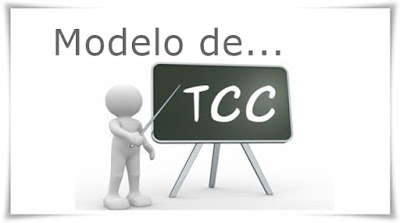
\includegraphics[scale=0.9]{img/ModeloImagem.jpg}
\caption{Modelo de Imagem \cite{pimentel1995}}
\label{modeloimg}
\end{figure}
 
	A Figura \ref{modeloimg} mostra um exemplo de como inserir uma imagem/figura e como fazer referência bibliográfica a mesma. 


Segundo \citeonline{marcoswagner_tese}, um exemplo de itens pode ser visto abaixo:

	\begin{itemize}
		\item Quanto as características da lesão:
		
	\begin{itemize}
		\item Tempo em que ocorreu a lesão:
		\item Extensão da lesão.
		\item Local da lesão.
	\end{itemize}
		\item Biografia do paciente:
		\item Idade.
		\item Diagnóstico. 
		\item Início e duração da terapia.
		\item Frequência e intensidade da terapia.
		\item Estado emocional.
		\begin{itemize}
			\item Motivação.
			\item Depressão.
		\end{itemize}
		\item Ambiente terapêutico.
		\item Comunicação.
		\item Condições físicas.
		\item Cognição; e
		\item Programa terapêutico.
	\end{itemize}




\section{Considerações Finais}
Tanto a seção Introdução como a seção Considerações Finais são opcionais na construção de um texto monográfico. Porém deve-se optar por um padrão. Coloca-se em todos os capítulos ou em nenhum...


\end{comment}
